Standardně jsou čísla v počítači uložena jako sled bitů v nějaké reprezentaci vyjadřující hodnotu. Tímto způsobem lze reprezentovat číslo jen s danou přeností a rozsahem, což je však v řadě případů dostačující. Čísla lze reprezentovat i naprosto přesně -- pomocí struktur je reprezentujícími a s nimi manipulujícími. I tyto samozřejmě musí být uloženy v paměti, v tomto případě se však nejedná o uložení hodnoty čísla, nýbrž se ukládá abstrakce, která číslo na požádání umí vygenerovat. Tento přístup nazýváme líným. Nejprve bude popsáno ukládání čísel jako hodnot a na jeho přesnost. Poté navrhneme struktury pro přesná čísla a nakonec budou ukázány existující knihovny.

\subsection{Čísla uložená jako hodnoty}
Paměť počítače většinou pracuje s tzv. \textit{bity}, paměťovými buňkami nabývajícími dvou rozlišitelných hodnot \cite{KepOS}. Ke kódování čísel se tedy používá výhradně dvojková soustava. Celá následující podkapitola pojednávající o uložení čísel jejich hodnotami je převzata z \cite{Knu02}.

\subsubsection{Vážený poziční kód}
Číslo v soustavě o základu $b$ lze dešifrovat následovně:
\begin{equation}
(\ldots a_2a_1a_0.a_{-1}a_{-2} \ldots )_b = \cdots + a_2b^2 + a_1b + a_0 + \frac{a_{-1}}{b} + \frac{a_{-2}}{b^2} + \cdots
\end{equation}kde čísla $a_n$ nazýváme číslice a symbol \uv{$.$} řádovou tečkou -- speciálně pak tečkou \textit{desetinnou} ($b=10$) nebo \textit{dvojkovou} ($b=2$).

\begin{example}[Převod z váženého pozičního kódu]
\begin{equation}
(101010.101)_2 = (42.625)_{10}
\end{equation}
\end{example}

\subsubsection{Záporná čísla}
V případě zápisu čísla váženým pozičním kódem lze strukturu pokrývající i záporná čísla přímočaře vytvořit přidáním příznaku (rozšířit jeho reprezentaci o jeden bit), zda se jedná o číslo kladné či nikoliv. V této reprezentaci lze vyjádřit zápornou i kladnou nulu. Tomutu kódování se říká kód \textit{velikostí a znaménkem (signed-magnitude)}.

Jinou možností je záporná čísla vnímat jako opak čísel kladných i na úrovni reprezentace, čili záporné číslo opačné ke kladnému v binární reprezentaci vypadá jako negace bitů daného kladného čísla. Opět zde vyvstává problém se zápornou nulou. Tomutu kódování se říká \textit{jedničkový doplněk (ones' complement)}.

Když od všech záporných čísel v jedničkovém doplňku odečteme číslo jedna, rozprostřeme čísla efektivně, tj. odpadne problém s dvojí reprezentací nuly. Tomutu kódování se říká \textit{dvojkový doplněk (two's complement)}.

\subsubsection{Plovoucí řádová tečka}
U váženého pozičního kódu známe přesně pozici řádové tečky -- je mezi číslicemi $a_0$ a $a_{-1}$. Alternativním přístupem je kódování s \textit{plovoucí} řádovou tečkou.

Plovoucí číslo je dáno uspořádanou dvojicí $\langle e,f\rangle = f * b^{e-q}$, kde $e$ nazýváme \textit{exponent} a $f$ \textit{zlomkovou částí (fraction)}. Čísla $b$ a $q$ jsou konstanty dané použitým typem, $b$ se nazývá \textit{základ} a $q$ \textit{přesah}.

\begin{example}[Plovoucí číslo -- jednoduchá přesnost]
Číslo s jednoduchou přesností (\textit{single} dle IEEE 754-1985, \textit{binary32} dle IEEE 754-2008) je uloženo v paměti jako 32b struktura. První bit je příznak znaménka, dalších 8 bitů je pro exponent a dalších 23 bitů pro fraction. Konstanty jsou ohodnoceny následovně: $q=127$, $b=2$. V \textit{C}, \textit{C++}, \textit{C\#} nebo \textit{Javě} se tento číselný datový typ nazývá \textit{float}, v \textit{Haskellu Float} a v \textit{Lispu} pak \textit{single-float} \cite{wiki:float}.
\begin{myfigure}{H}
\caption{Seřazení bitů v datovém typu binary32 \cite{wiki:file:binary32}}
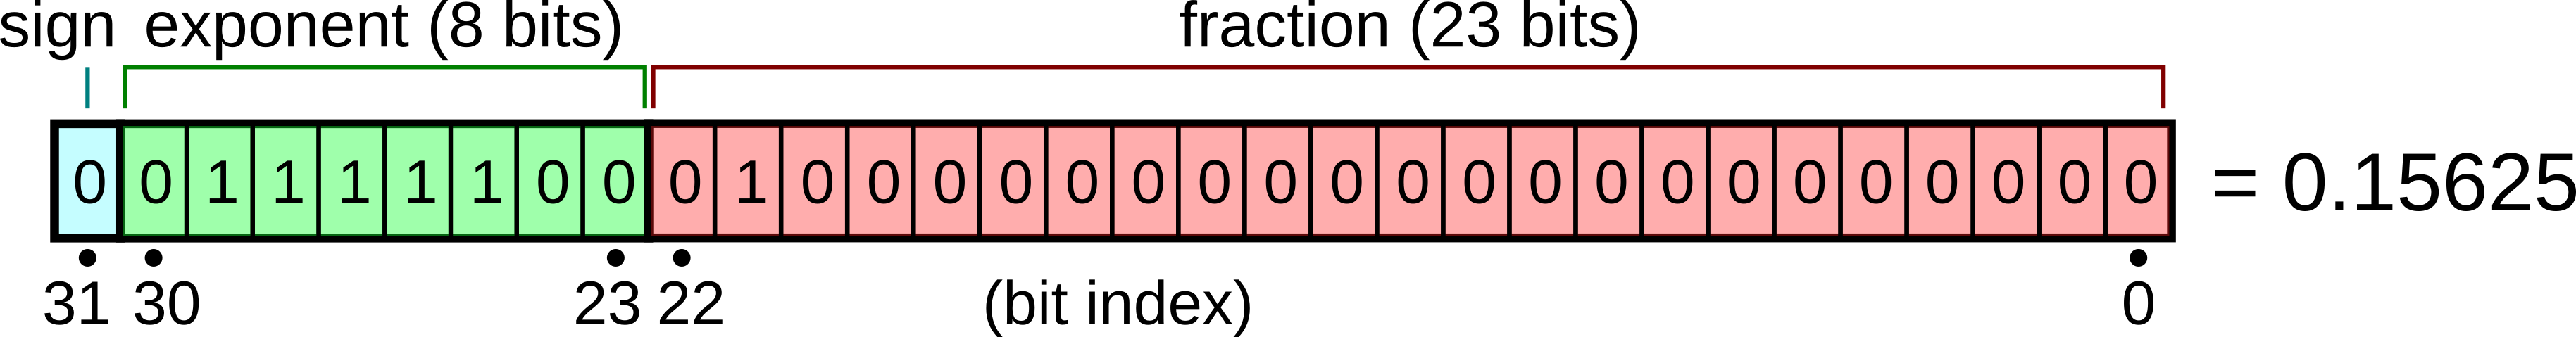
\includegraphics[width=\linewidth]{graphics/float.png}\label{obr:binary32}
32-bitový datový typ pro čísla s plovoucí řádovou tečkou je dle standardu uložen v konfiguraci $\langle s,e,f \rangle=\langle 1,8,23\rangle$.
\end{myfigure}
\end{example}

\subsection{Přesná reprezentace čísel jako hodnot}
Nyní se podívejme, jaká čísla uložená jako hodnoty považujeme za přesná. Projdeme opět všechny obory jako v první kapitole a poprvé propojíme matematickou teorii s informatickou realitou. Jako modelový jazyk nám poslouží C.

Všechny ukázky v této kapitole představují reálné chování představených datových typů na konkrétní AMD64 architektuře. Nejde teď tedy o žádnou teorii a jen ukazuji reálné limity. Na 128-bitové architektuře mohou být tyto limity jiné a typy použitelnější. Nicméně tato práce směřuje k přesným výpočtům rekurzivních čísel bez ohledu na architekturu.

\subsubsection{Přirozená čísla}
Přirozená čísla jsou uzavřena na operace sčítání a násobení. V počítači se jako hodnoty ukládají pomocí váženého pozičního kódu a tento má horní limit, jak velké číslo lze na dané architektuře uložit. Takto uložená přirozená čísla ovšem nejsou na operace uzavřena, protože může dojít k přetečení -- číslo ukládané se liší od čísla uloženého. Příklad tohoto chování vydíme na Obrázku \ref{obr:uinty}.
\begin{myfigure}{H}
\caption{Přirozená čísla v jazyce C}
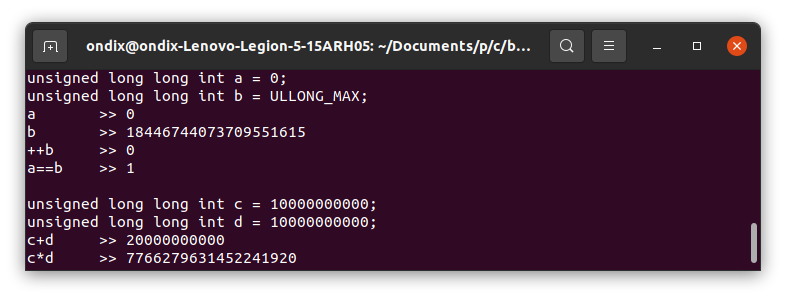
\includegraphics[width=\linewidth]{./graphics/uinty.png}\label{obr:uinty}
Největším datovým typem, který pracuje s přirozenými čísly je v jazyce C typ \texttt{unsigned long long int} a na 64-bitové architektuře umí uchovat čísla v intervalu $[0, 2^{64}-1]$. Na příkladu vidíme přetečení u inkrementace i násobení.
\end{myfigure}
Pokud ale ukládáme přirozené číslo v intervalu, ve kterém jej zvládne uložit datový typ jako hodnotu, můžeme ho považovat za přesné.

\subsubsection{Celá čísla}
Celá čísla jsou uzavřena na sčítání, odčítání a násobení. V paměti počítače se pak musí používat kódování záporných čísel jako hodnot, často jde o dvojkový komplement. Opět zde vyvstává problém s limity jakéhokoli hodnotového datového typu, totiž že vyjadřitelná čísla jsou ohraničená a hrozí přetečení (a i podtečení). Implementace celého čísla jako hodnoty tedy není na operace uzavřená (Obr. \ref{obr:inty}).
\begin{myfigure}{H}
\caption{Celá čísla v jazyce C}
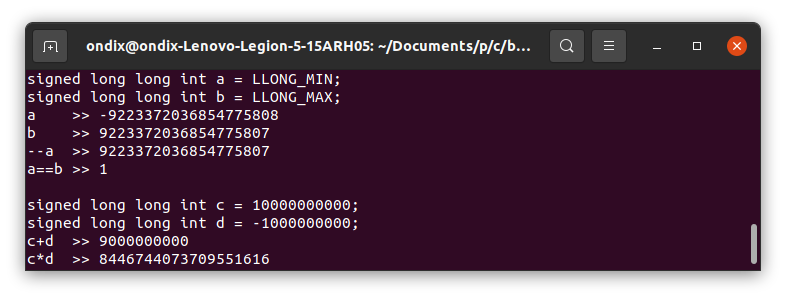
\includegraphics[width=\linewidth]{./graphics/inty.png}\label{obr:inty}
Nejširší datový typ jazyka C, který umí uložit celá čísla je \texttt{signed long long int}. Ten na 64-bitové architektuře zvládne uložit čísla z intervalu $[-2^{63}, 2^{63}-1]$. Na příkladu vidíme, že není uzavřen vůči operacím a že dochází k podtékání.
\end{myfigure}
Pakliže ukládáme celé číslo jako hodnotu, která se vejde do datového typu bez přetečení nebo podtečení, lze takto vyjádřené číslo považovat za přesné.

\subsubsection{Racionální čísla}
Racionální číslo se v jazyce C ukládá jako číslo s plovoucí řádovou tečkou. S~největší přesností se ukládá datový typ \texttt{long double}. Není specifikováno, jak má být přesný, pouze že má být minimálně tak přesný jako \texttt{double} \cite{wiki:LD}. Čísla, která jsou různá, ale kvůli zaokrouhlení se vyjádří jako stejná hodnota plovoucího čísla, jsou v~tomto směru potom nerozeznatelná. Každý plovoucí typ pak má garantovanou přesnost, na kterou by se různá čísla neměla reprezentovat stejně.

\begin{myfigure}{H}
\caption{Racionální čísla v jazyce C}
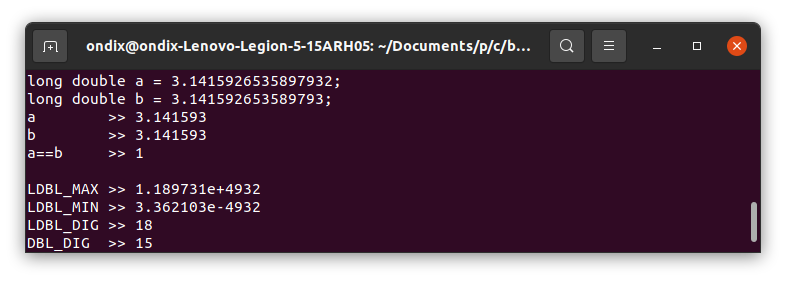
\includegraphics[width=\linewidth]{./graphics/floaty.png}\label{obr:floaty}
Nejrozsáhlejším datovým typem čísla s plovoucí řádovou tečkou je v jazyce C \texttt{long double}. Na příkladu vidíme, že jeho přesnost by měla být 18 desetinných míst, ale už na patnácti místech jsou dvě různá zapisovaná čísla zapsána stejně. Někde se tedy stala chyba a přesnost \texttt{long double} je stejná jako \texttt{double}, ale knihovna \texttt{float.h} to nereflektuje.
\end{myfigure}

Racionální čísla vyjádřená jako plovoucí můžeme považovat za přesná, pokud se nedostaneme mimo interval a přesnost stanovenou typem. Na Obrázku \ref{obr:floaty} vidíme, že rozsah datového typu \texttt{long double} je téměř $10^4$ řádů a přesnost je maximálně 15 desetinných míst. Čísla s plovoucí řádovou tečkou jsou nejlepší přiblížení k racionálním číslům, které lze vyjádřit jako hodnoty.
\subsection{Přesná reprezentace čísel jako struktur}
Již víme, že některá čísla lze přesně uložit jejich hodnotou. Narazili jsme ale na limity standardních datových typů, například přetékání nebo nedostatečná přesnost. Nyní se podíváme na filozofii reprezentace čísla nějakým referenčním typem, nikoli hodnotovým. Vynořuje se zde paralela s popisem čísel z první kapitoly, že stejné číslo lze vyjádřit několika symboly, i když jeho hodnota je pouze jedna. Pokusíme se tedy nyní podívat na tento druhý přístup a zjistíme, že takto reprezentovaná čísla umíme velmi dobře v počítači vyjadřovat. Struktury si budeme pouze představovat a nebudu tedy psát žádný konkrétní kód, jen se pokusíme vymyslet, jak by konkrétní struktury mohly pracovat. Stačí totiž jediná struktura, na které se shodneme, že může představovat číslo a pak už bude jasné, že může existovat i nějaká její implementace.

\subsubsection{Přirozená čísla}
Jak bylo řečeno v minulé podkapitole, přirozená čísla jsou uzavřena na sčítání a násobení, \texttt{unsigned int}y ovšem nikoli. Potřebovali bychom vymyslet strukturu, která zajistí, že dokáže reprezentovat jakékoli přirozené číslo. Jako hodnoty umíme na $n$ bytech uložit čísla $0$ až $2^n-1$. Nápad na přirozené číslo je rozumně upravovat toto $n$ a pak velikost čísla bude omezena jen velikostí paměti.

Struktura představující reálné číslo musí zajišťovat, že při operacích jeho hodnota nepřeteče. Pokud tedy dostane požadavek na násobení nebo sčítání, musí mít připravený další prostor a tam posunout bity, které by normálně přetekly. To by šlo zajistit tak, že ve svém pomyslném paměťovém prostoru bude vždy po provedení operace procházet svých levých $2^{n-1}$ bitů a pokud tam najde alespoň jednu jedničku, požádá o alokaci dalšího prostoru o velikost $2^n$, tedy zvedne $n$ o~jedna.

Pak už bude na operačním systému, kolik paměti bude moci struktuře přiřadit a tato paměť je vždy prakticky omezená, ale teoreticky je neomezená. Naši strukturu si tedy lze představit jako pouhý chytrý řadič bloků paměti za sebe. Pak lze \textit{naprosto přesně} zapsat jakékoli přirozené číslo. Paměťově toto není moc efektivní, ale je to funkční představa a nám teď stačí jen princip, jak by něco takového fungovat mohlo a optimalizaci necháváme až na konkrétní knihovny.

\subsubsection{Celá čísla}
U celých čísel je nápad velmi podobný jako u přirozených čísel. Kromě přetečení lze hrozí také podtečení, protože celá čísla musí být uzavřena i na odčítání. Vytvořme naši strukturu pro celé číslo jako dvojici přirozeného čísla a příznaku kladnosti.

Metody struktury pak budou jen nastavovat příznak kladnosti -- u násobení jako exklusivní disjunkci, odčítání je pak sčítání s negací příznaku a u sčítání se příznak nastaví podle většího čísla. Takto vytvořené struktury pak \textit{naprosto přesně} reprezentují jakékoli celé číslo.

\subsubsection{Racionální čísla}
Racionální čísla jsme definovali jako poměr celého a nenulového celého čísla. Racionální čísla (bez nuly) jsou uzavřená i na dělení. Zaveďme teď racionální číslo jako dvojici celých čísel s invariantem, že druhé číslo nesmí být nikdy nula a že obě čísla jsou nesoudělná.

Násobení bude fungovat jako násobení na složkách, dělení pak bude jen prohození obou složek druhého argumentu a následné násobení. Odčítání je opět sčítání s opačným číslem a sčítání musí najít společný jmenovatel a poté specificky přenásobovat jednotlivé operandy, ale složité to není.

Metody musí stále kontrolovat, zda nedochází k dělení nulou. Také po konci výpočtu musí zkrátit obě složky čísla. Predikát rovnosti dvou racionálních čísel kvůli podmínce nesoudělnosti je pak jednoduchý a je to rovnost na složkách.

Tato struktura je \textit{naprosto přesnou} reprezentací racionálních čísel. Jazyk Lisp se vydal cestou implementace racionálních čísel jako takto přesných a nabízí typ \texttt{ratio}.

\subsection{Reálná čísla}
Předchozí číselné obory lze tedy s dostatkem paměti naprosto přesně reprezentovat. To není málo. Zbývájí už \uv{jen} reálná čísla. Protože máme přesná racionální čísla, do reálných chybí už jen čísla iracionální. Těch je ale bohužel nepočitatelně mnoho, a tak nepůjdou vytvořit z přirozených čísel nabalováním struktur jako předchozí obory (důkaz, že toto není jednoduché je existence práce, kterou právě čtete).

Nic jiného ale v paměti, která pracuje s diskrétními hodnotami neumíme vytvořit. Přepneme teď přístup. Dosud jsme mluvili o \textit{naprosto přesných} číslech, teď ovšem přijmeme názor, že struktura vyjadřující přesné číslo může být i taková, která počítá jen přibližná čísla, ale nastavitelně vzdálená od přesné hodnoty, kterou ovšem neznáme. Takových čísel je počitatelně mnoho a říkáme jim čísla rekurzivní. Ve skutečnosti je právě hranice mezi racionálními čísly a rekurzivními čísly ta velká bariéra, která odděluje svět, kde vše funguje relativně jednoduše a ten, kde je všechno o řád těžší.

Na začátku této podkapitoly ještě zůstaneme v myšlenkové rovině a budeme si abstraktní struktury představovat, ve druhé polovině potom ukážu, že některé struktury pro přesnou reprezentaci rekurzivních čísel existují.

\subsubsection{Představa}\label{kap:predstava}
Než struktury definovat imperativně pomocí definic, jak by co měla implementovat se spíše pokusím o definici struktury deklarativně, čili pomocí jejích vlastností, které by měla splňovat.

Abstraktní struktura reprezentující reálné číslo by měla umožnit
\begin{itemize}
\item{jeho vyčíslení -- když struktura existuje, pak po zavolání vhodného nástroje je výsledkem hodnota, kterou tato struktura představuje;}
\item{přesnost -- i když má číslo nekonečný rozvoj nebo je velmi velké, abstrakce umožňuje jeho vyčíslení na danou přesnost v konečném čase;}
\item{podporovat matematické operace -- ve smyslu kapitoly \ref{operace_s_cisly};}
\item{podporovat matematické funkce -- ve smyslu kapitoly \ref{funkce_cisel};}
\item{být vracena jako výsledek funkce -- mít jasně popsanou strukturu, aby se dala rozšiřovat funkčnost;}
\item{být použita jako argument nějaké funkce -- typicky funkce pro vyčíslení.}
\end{itemize}

První dvě podmínky jsou přímo esenciální -- zajišťují, že abstrakce mohou reprezentovat reálná čísla na libovolnou (kladnou) přenost. Kdykoli budu potřebovat číslo dané nějakou abstrakcí, zavolám příslušnou funkci ještě s nějakým parametrem $\varepsilon$ reprezentujícím přesnost, na kterou toto číslo potřebuji. Obecně totiž nemusí být výsledkem vyčíslovací funkce přesná hodnota hledaného čísla, avšak díky těmto podmínkám budu výsledku vzdálen maximálně o zadanou hodnotu odchylky. To je tedy význam onoho \textit{přesného} v názvu této práce -- výsledkem enumerace nikdy nemusí být naprosto přesné číslo, ale číslo, které je od výsledku vzdálené o jasně definovanou hodnotu a tento výpočet skončí. Když budu uvažovat nějakou strukturu $s_x$ přesně vyjadřující nějaké číslo $x$, zavolám vyčíslovací funkci $enum$ a jako argumenty použiji tuto strukturu a libovolné kladné $\varepsilon$, pak bych měl dostat výsledek $enum(s_x, \varepsilon)$ splňující nerovnost
\begin{equation}
|enum(s_x, \varepsilon)-x| \leq \varepsilon.
\end{equation}

Druhé dvě podmínky vštěpují dané struktuře reprezentující reálná čísla vlastnosti reálných čísel a sice že s nimi jde sčítat, násobit atp. a že mohou být argumentem nějaké matematické funkce. Jistě nejde o to tyto struktury vkládat do stejných operací jako si představujeme s normálními čísly, například ve výrazu $3+4$ nechceme operandy nahrazovat abstraktními strukturami a očekávat správný výsledek, nýbrž chceme existenci ekvivalentní operace pro tyto struktury. To nutně neznamená, že musí být skutečně někde implementována, ale potřebujeme docílit stavu, kdy existence této není dokazatelně vyloučena.

Třetí a poslední dvě podmínky jsou spíše návod pro praktické použití těchto hypotetických struktur, aby se s nimi dalo smysluplně pracovat. To vlastně znamená, že musí být elementy prvního řádu (\textit{first-class citizen}), čili implementovány jako niterná součást použitého jazyka a ne jako svébytná konstrukce, která sice funguje, ale je nekompatibilní s jazykem svého vzniku, takže je vlastně nepoužitelná, uživatelsky nerozšiřitelná.

\subsubsection{Existující nástroje}\FloatBarrier
Nyní se podíváme, co na poli vyčíslování reálných čísel existuje v současné době.
\paragraph{Mpmath \cite{mpmath}}
\texttt{mpmath} je velmi rozsáhlá knihovna pro Python. Je publikována pod licensí BSD a je dosažitelná i pomocí \texttt{pip}u. Kromě základní funkčnosti pro výpočet funkcí a operací s čísly jsou implementovány i funkce pro výpočet funkcí intervalů, určitých integrálů, podpora tvorby grafů a mnoho dalšího. Dokumentace je velice hezky zpracovaná se spoustou příkladů. Přesnost se nastavuje proměnnou \texttt{mp.dps}. Jde o počet vypisovaných míst. Knihovna oplývá tolika možnostmi, že dokonce existuje stránka pro výpočet Ludolfova čísla sty možnými one-linery. Knihovna používá tři vlastní datové typy a sice \texttt{mpf} pro reálná čísla, \texttt{mpc} pro komplexní čísla a \texttt{matrix} pro matice.

\begin{myfigure}{}
\caption{Používání knihovny \texttt{mpmath}}
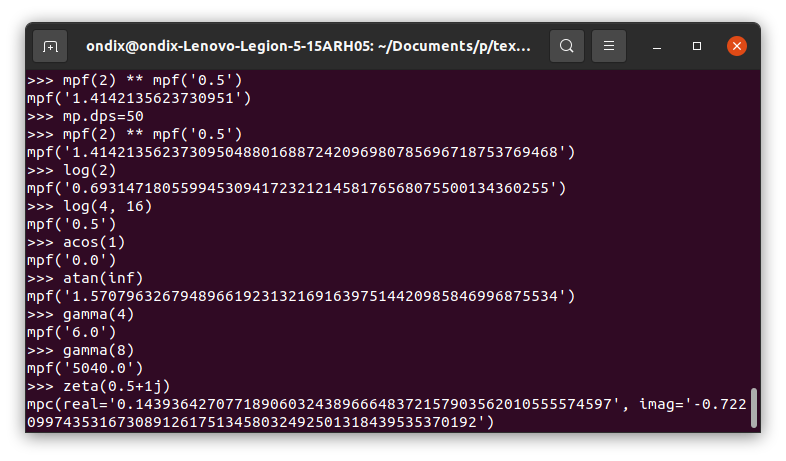
\includegraphics[width=\linewidth]{./graphics/mpmath.png}\label{obr:mpmath}
Vidíme, že struktura \texttt{mpf} podporuje matematické operace, na příkladu je odmocnina ze dvou. Ta je ve dvou provedeních, s defaultní přesností a s nastavenou na 50. Dále vidíme matematické funkce, jmenovitě logaritmus, cyklometrické, gamma a Riemannovu zeta funkci. Na jejím vstupu i výstupu vidíme komplexní číslo.
\end{myfigure}

\paragraph{JScience \cite{jscience}}
\texttt{JScience} je knihovna pro jazyk Java. Její část pro práci s jednotkami se dostala do knihovny \texttt{javax}. Knihovna je široce rozkročena. Přináší podporu pro porovnávání a počítání jednotek z fyziky, geografie nebo ekonomie. Z matematiky je zde podpora pro jednoduchou symbolickou analýzu a strukturální algebru. Nás nejvíce zajímá část \texttt{org.jscience.mathematics.number}. Zde jsou zajímavé 3 datové typy a to \texttt{Real} umožnující základní výpočty s nastavitelnou přesností, \texttt{LargeInteger} ukládající velká celá čísla a \texttt{Rational} ukládající dvojice \texttt{LargeInteger}ů a umožňující jejich implicitní usměrňování a základní matematické operace.

\begin{myfigure}{}
\caption{Používání knihovny \texttt{JScience}}
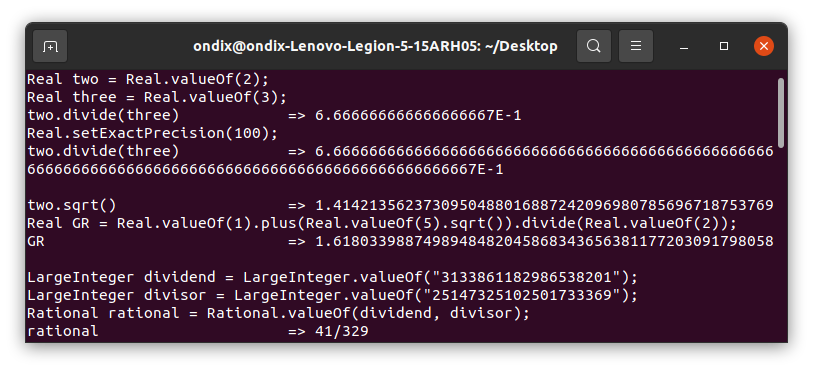
\includegraphics[width=\linewidth]{./graphics/jscience.png}\label{obr:jscience}
Vidíme používání třídy \texttt{Real}. Operace jsou použitelné jako metody, nikoli operátorem. Vidíme nastavování přesnosti, výpočet druhé odmocniny, zlatého řezu a zlomkové struktury s implicitním krácením.
\end{myfigure}

\paragraph{GNU Multiple Precision Arithmetic Library \cite{wiki:gmp} (GMP)}
\texttt{GMP} je knihovna pro jazyk C. Datový typ \texttt{mpz\_t} představuje celé číslo, u kterého nehrozí přetečení nebo podtečení. Zlomky velkých čísel představuje \texttt{mpq\_t} a operace podporují usměrňování. Přesný ekvivalent čísla s plovoucí řádovou tečkou představuje \texttt{mpf\_t}. Minimální počet bytů, ve kterém je uložen v paměti se nastavuje funkcí \texttt{mpf\_set\_default\_prec}. Všechny typy implementují základní matematické operace. Protože je GMP součástí projektu GNU a protože je to knihovna pro C, je velmi mnoho nadstavbových knihoven, které její funkcionalitu využívají a rozšiřují. Z C-čkových jmenujme například \texttt{GNU MPFR}, která na je na GMP přímo založena \cite{wiki:mpfr} a přináší matematické funkce floatů, nebo \texttt{MPIR} -- paralelní projekt odtrhnuvší se od vývoje GMP a jdoucí svojí cestou, přesto snažící se implementovat rozhraní GMP, aby byly zastupitelné \cite{wiki:mpir}. Dále existují wrappery pro kompatibilitu s jinými jazyky a tudíž je GMP velmi rozšířená, ač se to nemusí uživateli zdát. Například pro platformu .NET je to knihovna \texttt{Math.GMP.Native}, pro Python \texttt{gmpy}, pro R \texttt{gmp} a takových příkladů najdeme hodně.

\begin{myfigure}{}
\caption{Používání knihovny \texttt{GMP}}
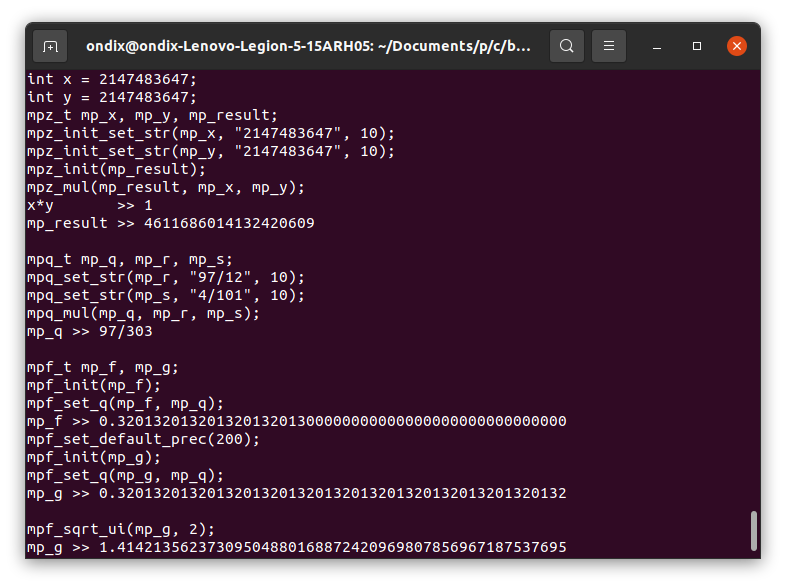
\includegraphics[width=\linewidth]{./graphics/gmp.png}\label{obr:gmp}
Na příkladu vidíme nejprve porovnání násobení klasických intů versus struktur typu \texttt{mpz\_t}. U intů dojde k přetečení, u mpz nikoli. Dále vidíme práci se zlomky, jejich inicializaci ze stringu a násobení. Nakonec vidíme základní operace s typem \texttt{mpf\_t}, protějškem čísel s plovoucí řádovou tečkou.
\end{myfigure}

\paragraph{Class Library for Numbers \cite{wiki:CLN} (CLN)} \texttt{CLN} je knihovna pro jazyk C++. Je také zdarma šířená pod licensí GPL. Implementuje jak čísla s~plovoucí řádovou tečkou, tak racionální čísla jako zlomky, navíc komplexní čísla. Za přesné se považují racionální čísla a komplexní čísla s přesnou imaginární i reálnou částí. Plovoucí čísla pak typově přesně kopírují Lispovské a dají se tedy použít k Lispovským implementacím. Tím pádem se zkratka CLN dá chápat i jako \uv{Common Lisp Numbers}.

\begin{myfigure}{}
\caption{Implicitní používání knihovny \texttt{CLN}}
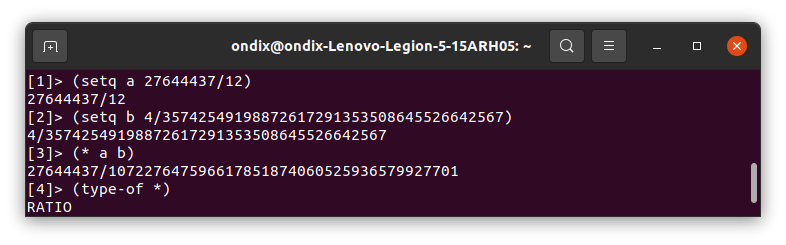
\includegraphics[width=\linewidth]{./graphics/clisp.png}\label{obr:clisp}
Knihovnu CLN používá CLisp, interpret jazyka Lisp. Využívá implementace čísel. Příklad ukazuje, že se zlomky zkracují, aniž by bylo třeba k tomu voláním vybízet, ale děje se automaticky. Že je CLisp založen na CLN usuzuji podle osoby Bruna Heible-a, který figuruje jako autor jak u CLN, tak u CLisp-u.
\end{myfigure}

\paragraph{Computable-reals \cite{gh:cr}}\label{kap:computable-reals}
\texttt{computable-reals} je Lispovská knihovna. Je volně ke stažení a dokonce k dostání pomocí \texttt{quicklisp}u. Podporuje základní funkcionalitu. Její funkce poznáme tak, že končí koncovkou \texttt{-r}. Vracené výsledky nejsou čísla, ale vlastního typu \texttt{C-REAL}. Defaultně se tisknou výsledky na 20 míst, ale nastavením proměnné \texttt{*print-prec*} se tento počet dá měnit \cite{lpb:numbers}. Kromě odmocniny jsou zde třeba základní násobky čísla $\pi$, logaritmy, mocniny, základní goniometrické funkce, arcus tangens. Knihovna se používá jako kalkulačka s nastavitelnou přesností.

\begin{myfigure}{}
\caption{Používání knihovny \texttt{computable-reals}}
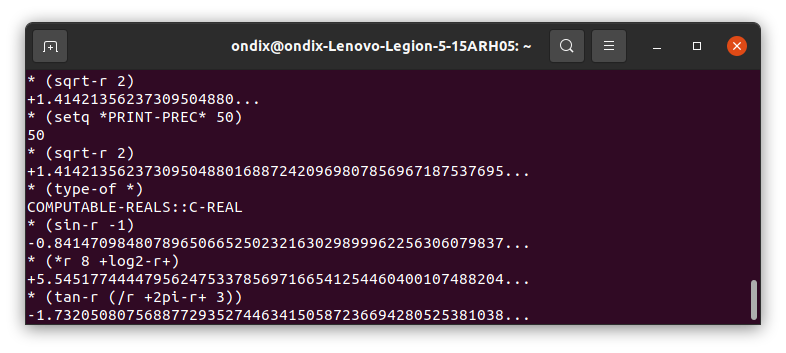
\includegraphics[width=\linewidth]{./graphics/computable-reals.png}\label{obr:computable-reals}
Na příkladu vidíme výpis odmocniny ze dvou na různé přesnosti, operace násobení a  několik matematických funkcí.
\end{myfigure}\FloatBarrier

\paragraph{Cíl práce}
Tolik tedy k strukturám již nyní implementujícím čísla a jejich operace, případně funkce. V některých implementacích se jedná o třídy, v jiných jde o strukturované datové typy. V následujícím textu se pokusíme navázat tam, kde končí naprostá přesnost nad racionálními čísly jazyka Lisp a naprogramujeme knihovnu přinášející některá iracionální čísla.

V této práci nám jde o přesnost a nikoli o rychlost a proto jako nativní typy budu používat právě zlomky, ačkoli pro rychlé operace s desetinnými čísly se používají plovoucí čísla, které mají často i hardwarovou podporu v jednotce FPU. Ostatně proto jsou v Lispu i plovoucí typy \cite{PS:PCL}.

K programování jsem jako textový editor použil \textit{Visual Studio Code} s rozšířením \textit{Rainbow Brackets} a jako překladač \textit{SBCL}.